\documentclass[11pt,a4paper]{article}
\usepackage[hyperref]{acl2018}
\usepackage{times}
\usepackage{latexsym}

\usepackage[letterpaper]{geometry}
%\usepackage{amta2016}
\usepackage{url}
\usepackage{natbib}
\usepackage{layout}

\usepackage{algorithm}% http://ctan.org/pkg/algorithms
\usepackage{algpseudocode}% http://ctan.org/pkg/algorithmicx

\usepackage{graphicx}
\usepackage{amsmath}
\DeclareMathOperator*{\argmax}{argmax}

\newcommand{\confname}{AMTA 2016}
\newcommand{\website}{\protect\url{http://www.amtaweb.org/}}
\newcommand{\contactname}{research track co-chair Lane Schwartz}
\newcommand{\contactemail}{lanes@illinois.edu} 
\newcommand{\conffilename}{amta2016}
\newcommand{\downloadsite}{\protect\url{http://www.amtaweb.org/}}
\newcommand{\paperlength}{$12$ (twelve)}
\newcommand{\shortpaperlength}{$6$ (six)}

%% do not add any other page- or text-size instruction here

\parskip=0.00in

\begin{document}

% \mtsummitHeader{x}{x}{xxx-xxx}{2016}{45-character paper description goes here}{Author(s) initials and last name go here}
\title{\bf Focusing on Fast Neural Network Inference}  

\author{\name{\bf Hieu Hoang} \hfill  \addr{hieu@hoang.co.uk}\\ 
        \addr{}
\AND
       \name{\bf Tomasz Dwojak} \hfill \addr{???}\\
        \addr{Adam Mickiewicz University}
\AND
       \name{\bf Kenneth Heafield} \hfill \addr{???}\\
       %\name{\bf Kenneth Heafield} \hfill \addr{kheafiel@inf.ed.ac.uk}\\
        \addr{University of Edinburgh, Scotland}
}

\maketitle
\pagestyle{empty}

\begin{abstract}

This paper describe the submissions to the efficiency track for GPUs by members of the University of Edinburgh, Adam Mickiewicz University, Tilde and University of Alicante. We focus on efficient implementation of the recurrent deep-learning model as implemented in Amun, the fast inference engine for neural machine translation. We improve the performance with an efficient mini-batching and maxi-batching algorithm. Translation speed was also reduced by fusing the softmax operation with the beam seach algorithm.


\end{abstract}

\section{Introduction}
\label{sec:Introduction}

As neural machine translation (NMT) models have become the new state-of-the-art, the challenge is to make their deployment efficient and economical. This is the challenge that this shared task is shining a spotlight on.

It is tempting to use a general purpose deep-learning toolkit such as Tensorflow or Pytorch to train and do the the inference where faster translation could be obtained by tuning parameters within the toolkit, and choosing fast models. %We believe this is the approach most other submissions have taken.

We take an opposing approach by using and enhancing a custom inference engine, Amun~\citep{junczys2016neural}, which we developed on the premise that fast deep-learning inference is an issue that deserves dedicated tools which are not compromised by other objectives such as training or support for multiple models. As well as delivering on the useful goal of fast inference, it can serve as a test-bed for novel ideas on neural network inference, and is useful as a means to explore the upper limit of the possible speed for a particular model and hardware. That is, Amun is an inference-only engine that supports a limited number of NMT models that put fast inference on modern GPU above all other considerations. %The consequence of this focused approach can be seen in the results of the shared task ???.

We submitted two systems to this year's shared task for the efficient translation on GPU. Our first submission was tailored to be as fast as possible while being above the baseline BLEU score. Our second submission trade some of the speed of first submission to return good quality translation.

We will describe below our experimental setup as well as the enhancements to Amun that we feel enabled it to achieve its outstanding speed.


\section{Improvements}

We desribe the main enhancements to Amun since the original 2016 publication.

\subsection{Batching}

The use of mini-batching is critical for fast model inference. The size of the batch is determined by the number of inputs sentences to the encoder in an encoder-decoder model. However, the number of batches during decoding can vary as some sentences have completed translating or the beam search add more hypotheses to the batch.

It is tempting to ignore these considerations, for example, by always decoding with a constant batch and beam size and ignoring hypotheses which are not needed but this comes at a cost of lower translation speed due to wasteful processing.

The Amun engine implements an efficient batching algorithm that takes into account the actual number of hypotheses that needs to be decoded at each decoding step, Figure~\ref{algo:Mini-batching}.

\begin{algorithm}
\begin{algorithmic}
\Procedure{Batching}{encoded records $i$}

\State Create batch $b$ from $i$

\While{$b$ is not empty} 
  \State $b' \gets$ DecodeAndBeamSearch($b$)
  \State $b \gets \emptyset$
  
  \ForAll{hypo $h$ in $b'$}
    \If{$h \neq \textless/s \textgreater$  }
      \State Add $h$ to $b$
    \EndIf
  \EndFor
\EndWhile

\EndProcedure

\end{algorithmic}
\caption{Mini-batching}
\label{algo:Mini-batching}
\end{algorithm}


\subsection{Softmax and Beam Search Fusion}

Most NMT more predict a large number of classes in their output layer, corresponding to the number of words or subword units in their target language. For example, ~\citet{sennrich-haddow-birch:2016:P16-12} experimented with target vocabulary sizes of 60,000 and 90,000 sub-word units. This makes the output layer of NMT models very computationally expensive. Figure~\ref{fig:pie-time-europarl} shows the breakdown of amount of time during translation our NMT system; nearly 70\% of the time is involved in the output layer. We describe the steps to fuse the operations to improve efficiency.
\begin{figure}
\centering
\begin{tabular}{cc}
{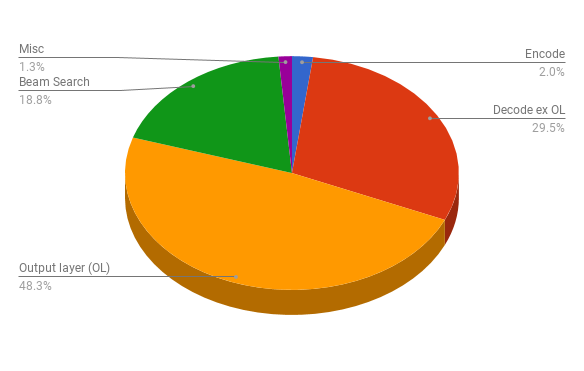
\includegraphics[scale=0.3]{pie-time-europarl.png}} 
\end{tabular}
\caption{Proportion of time spent during translation (Europarl test set)}
\label{fig:pie-time-europarl}
\end{figure} 

The output layer of most deep learning models consist of the following steps
\begin{enumerate}
   \item \vspace{-2 mm} multiplication of the weight matrix with the input vector $p = w x$
   \item \vspace{-2 mm} addition of a bias term to the resulting scores $p = p + b$
   \item \vspace{-2 mm} applying the activation function, most commonly softmax $ p_i = \exp(p_i) / \sum \exp(p_i) $
   \item \vspace{-2 mm} a beam search for the best (or n-best) output classes $\argmax_i p_i$
\end{enumerate}

In models with a small number of classes such as binary classification, the computational effort required is trivial and fast but this is not the case for the large number of classes found in typical NMT models.

We leave step 1 for future work and focus on the last three steps, the outline for which are shown in Algorithm~\ref{algo:original-softmax-beamsearch}. For brevity, we show the algorithm for 1-best, a beam search of the n-bests is a simple extension of this.

\begin{algorithm} 
\begin{algorithmic}

\Procedure{AddBias}{vector $p$, bias vector $b$}
\ForAll{$p_i$ in $p$}
  \State $p_i \gets p_i + b_i$
\EndFor 
\EndProcedure

\State

\Procedure{Softmax}{vector $p$}

\Comment{calculate max for softmax stability}
\State $max \gets - \infty$ 
\ForAll{$p_i$ in $p$}
  \If{$p_i > max$}
    \State $max \gets p_i$
  \EndIf
\EndFor

\Comment{calculate denominator} 
\State $sum \gets 0$ 
\ForAll{$p_i$ in $p$}
  \State $sum \gets sum + \exp(p_i - max)$
\EndFor

\Comment{calculate softmax}
\ForAll{$p_i$ in $p$}
  \State $p_i \gets \frac{\exp(p_i - max)}{sum} $
\EndFor 

\EndProcedure

\State

\Procedure{Find-Best}{vector $p$}

\State $max \gets - \infty$ 
\ForAll{$p_i$ in $p$}
  \If{$p_i > max$}
    \State $max \gets p_i$
    \State $best \gets i$
  \EndIf
\EndFor 

\Return $max$, $best$

\EndProcedure

\end{algorithmic}
\caption{Original softmax and beam Search Algorithm}
\label{algo:original-softmax-beamsearch}
\end{algorithm}


As can be seen, the matrix p is iterated over five times - once to add the bias, three times to calculate the softmax, and once to search for the best classes. We propose fusing the three functions into one kernel, a popular optimization technique~\citep{Guevara2009EnablingTP}, making use of the following observations.

Firstly, softmax and $\exp$ are monotonic functions, therefore, we can move the search for the best class from FIND-BEST to SOFTMAX, at the start of the kernel.

Secondly, we are only interested in the probabilities of the best classes. Since they are now known at the start of the kernel, we compute softmax only for those classes.

\begin{algorithm}
\begin{algorithmic}
\Procedure{Fused-Kernel}{vector $p$, bias vector $b$}

\Comment{add bias, calculate $max$ \& $argmax$}

\State $max \gets - \infty$ 
\State $sum \gets 0$ 

\ForAll{$p_i$ in $p$}
  \State $p_i' \gets p_i + b_i$  
  \If{$p_i' > max$}
    \State $\Delta \gets max - p_i'$
    \State $sum \gets \Delta \times sum + 1 $
    \State $max \gets p_i'$
    \State $best \gets i$
  \Else
    \State $sum \gets sum + \exp(p_i' - max)$
  \EndIf
\EndFor

\Return $\frac{1}{sum}$, $best$ 

\EndProcedure
\end{algorithmic}

\caption{Fused softmax and beam search}
\label{algo:Fused Kernel}
\end{algorithm}

Thirdly, the calculation of $max$ and $sum$ can be accomplished in one loop by adjusting $sum$ whenever a higher $max$ is found during the looping:
\begin{eqnarray*}
sum & = & e^{x_t - max_b} + \sum_{i=0...t-1}{e^{x_i - max_b}} \\
    & = & e^{x_t - max_b} + \sum_{i=0...t-1}{e^{x_i - max_a + \Delta}}  \\
    & = & e^{x_t - max_b} + e^{\Delta} \times \sum_{i=0...t-1}{e^{x_i - max_a}} 
\end{eqnarray*}
where $max_a$ is the original maximum value, $max_b$ is the new, higher maximum value, ie. $max_b > max_a$, and $\Delta = max_a - max_b$. The outline of our function is shown in Algorithm~\ref{algo:Fused Kernel}.

In fact, a well known optimization is to skip softmax altogether and calculate the argmax over the input vector, Algorithm~\ref{algo:Argmax only}. This is only possible for beam size 1 and when we are not interested in returning the softmax probabilities.

\begin{algorithm}
\begin{algorithmic}
\Procedure{Fused-kernel-1-best}{vector $p$, bias vector $b$}

\State $max \gets - \infty$ 
\ForAll{$p_i$ in $p$}
  \If{$p_i + b_i > max$}
    \State $max \gets p_i + b_i$
    \State $best \gets i$
  \EndIf
\EndFor

\Return $best$ 

\EndProcedure

\end{algorithmic}
\caption{Find 1-best only}
\label{algo:Argmax only}
\end{algorithm}

%These changes do not reduce the asymptotic runtime of our algorithm, which remains at $\mathcal{O}(|p|)$, but it does bring the number of iterations over $p$ down from 5 to 1. In practise, this has a significant affect on inference speed.

\subsection{Half-Precision}

Reducing the number of bits needed to store floating point values from 32-bits to 16-bits promises to increase translation speed through faster calculations and reduced bandwidth usage. 16-bit floating point operations are supported by the GPU hardware and software available in the shared task.

In practise, however, efficiently using half-precision value requires a comprehensive redvelopment of the GPU code. We therefore make do with using the GPU's Tensor Core fast matrix multiplication routines which transparently converts 32-bit float point input matrices to 16-bit values and output a 32-bit float point product of the inputs.

\section{Experimental Setup}
\label{sec:Experimental Setup}

Both of our submitted systems uses the sequence-to-sequence model similar to that described in ~\citet{sennrich-haddow-birch:2016:P16-12}, containing a bidirectional RNN in the encoder and a two-layer RNN in the decoder. We use BPE to adjust the vocabulary size.

We used a variety of GPUs to train the models but all testing was done on an Nvidia V100. Translation quality was measured using BLEU, specifically multi-bleu as found in the Moses toolkit. The validation and test sets provided by the shared task organisers were used to measure translation quality, but a 50,000 sentence subset of the training data was used to measure translation speed to obtain longer, more accurate measurements.

\subsection{GRU-based system}

Our first system uses gated recurrent units (GRU) throughout, trained with Marian, but submitted both systems using the Amun inference engine.

We experimented with varying the vocabulary size and the RNN state size before settling for a vocabulary size of 30,000 (for both source and target language) and 256 for the state size, Table~\ref{tab:BLEU for newstest2014}.

\begin{table}
\begin{center}
\begin{tabular}{|l|r|r|r|} \hline
		& \multicolumn{3}{|c|}{\emph{State dim}}	\\ \hline	
Vocab size	& 256	& 512	& 1024 \\ \hline
1000 		& 12.23 &	& 12.77 \\ 
5000		& 16.79	&  	& 17.16 \\ 
10,000		& 18.00	& 	& 18.19 \\
20,000		& -	&	& 19.52 \\ 
30,000		& 18.51	& 19.17	& 19.64 \\ \hline
\end{tabular}
\end{center}
\caption{Validation set BLEU (newstest2014) for GRU-based model}
\label{tab:BLEU for newstest2014}
\end{table}

After further experimentation, we decided to use sentence length normalization and NVidia's Tensor Core matrix multiplication which increased translation quality as well as translation speed. The beam was kept at 1 throughout for the fastest possible inference.

\subsection{mLSTM-based system}

Our second system uses multiplicative-LSTM in the encoder and the first layer of a decder, and a GRU in the second layer, using an extension of the Nematus toolkit which supports such model. We trained 2 systems with differing vocabulary sizes and varied the beam sizes before choosing the the settings that produces good translation quality on the validation set, Table~\ref{tab:mLSTM BLEU - vocab sizes}. 

\begin{table}
\begin{center}
\begin{tabular}{|l|r|r|} \hline
		& \multicolumn{2}{|l|}{\emph{Vocab size}}	\\ \hline	
Beam size	& 40,000	& 50,000 \\ \hline
1 		& 23.45		& 23.32	\\ 
2		& 24.15		& 24.04	\\
3		& 24.48		&  	\\
4		& 24.42		& 	\\
5		& 24.48		& 	\\ \hline
\end{tabular}
\end{center}
\caption{Validation set BLEU for mLSTM-based model}
\label{tab:mLSTM BLEU - vocab sizes}
\end{table}

\section{Result}
\label{sec:Result}

\subsection{Batching}

Using batching can increase the translation speed by over 20 times in Amun and shows little degradation with larger batch sizes, Figure~\ref{fig:batch-size}. This contrast with using the Marian, which uses a simpler batching algorithm, where the speedup is approximately 16 times and inference speed slows down when the batch size is above 1000.

\begin{figure}
\centering
\begin{tabular}{cc}
{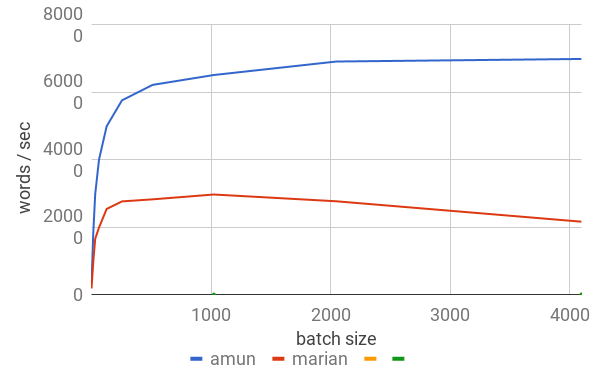
\includegraphics[scale=0.3]{batch-size.png}} 
\end{tabular}
\caption{Actual batch size during decoding}
\label{fig:batch-size}
\end{figure} 

The efficiency of Amun's batching algorithm can be seen by observing the time taken for each decoding step in a batch of sentence, Figure~\ref{fig:decode-step}. Amun's decoding becomes faster as sentences finish translating. By contrast, Marian's decoding time stays relatively constant.

\begin{figure}
\centering
\begin{tabular}{cc}
{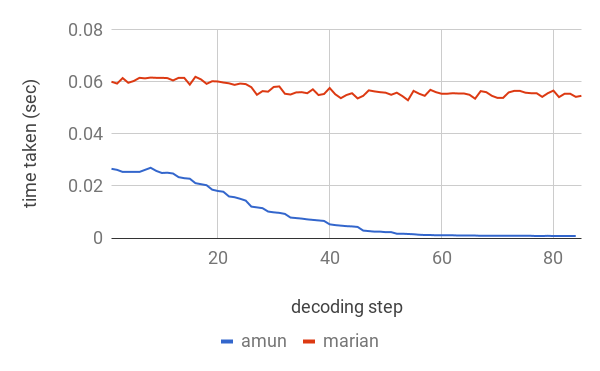
\includegraphics[scale=0.3]{decode-step.png}} 
\end{tabular}
\caption{Time taken for decoding each for a batch of 1280 sentences}
\label{fig:decode-step}
\end{figure} 

\subsection{Softmax and Beam Search Fusion}

////////////////////////////////////////////////////////////////


We have identified two areas where typical NMT models differ significantly from other deep-learning models that impact on their inference speed. Firstly, NMT models usually contains a large number of output classes, corresponding to the output vocabulary. Secondly, rather than a single label, the output from machine translation models is a sequence of class labels that makes up the words or sub-words in the target sentence. Target sentence lengths are unpredictable, leading to inefficiencies during batch processing. We provide solutions for each of these issues which together increase batched inference speed by up to 57\% on modern GPUs without affecting model quality.

We examine two areas that are critical to fast NMT inference where the models differ significantly from other deep-learning models. We believe the optimizations of these models have been overlooked by the general deep-learning community.



Even with sequence-to-sequence NMT models, target sentence lengths will still differ even for similar length inputs, compromising decoding performance. Figure~\ref{fig:batch-size} shows the actual batch size during decoding with a maximum batch size of 128; the batch was full in only 42\% of decoding iterations.

\begin{figure}
\centering
\begin{tabular}{cc}
{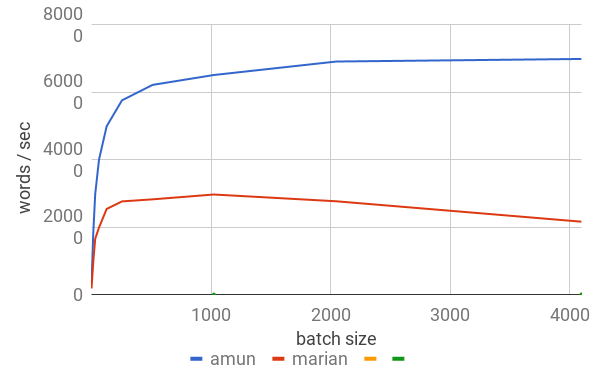
\includegraphics[scale=0.3]{batch-size.png}} 
\end{tabular}
\caption{Actual batch size during decoding (Europarl test set)}
\label{fig:batch-size}
\end{figure} 

We will propose an alternative batching algorithm to increase the actual batch size during decoding without the problems associated with mini-batching and maxi-batching.

\section{Prior Work}

Deep-learning models has been successfully used on many machine learning task in recent years in areas as diverse as computer vision and natural language processing. This success have been followed by the rush to put these model into production. The computational resources required in order to run these models has been challenging but, fortunately, there has been a lot work to meet this challenge.

Hardware accelerators such as GPUs are very popular but other specialized hardware such as custom processors~\citep{DBLP:journals/corr/JouppiYPPABBBBB17} and FPGA~\citep{DBLP:journals/corr/LaceyTA16} have been used. Hardware-supported reduced precision is also an ideal way to speed up model inference~\citep{DBLP:journals/corr/abs-1710-03740}.

Simpler, faster models have been created that are as good, or almost as good, as more slower, more complex models~\citep{DBLP:journals/corr/BahdanauCB14}. Research have also gone into smaller, faster models that can approximate slower, bigger models~\citep{DBLP:conf/emnlp/KimR16}. Some models have been justified as more suited for the parallel architecture of GPUs~\cite{DBLP:journals/corr/VaswaniSPUJGKP17}~\cite{gehring2017convs2s}.

The speed of the softmax layer when used with large vocabularies have been looked at in~\citet{DBLP:journals/corr/GraveJCGJ16} but there have been many other attempts at faster softmax, for example~\citet{DBLP:journals/corr/abs-1301-3781}, ~\citet{Zoph-2016}.

There has been surprisingly little work on batching algorithms, considering its critical importance for efficient deep-learning training and inference. ~\citet{Neubig-autobatching} describe an novel batching algorithm, however, its aim is to alleviate the burden on developers of batching models rather than faster batching.

Our paper follows most closely on from ~\citet{DBLP:conf/emnlp/Devlin17} which achieved faster NMT inference mainly by novel implementation of an existing model. However, we differ by focusing on GPU implementation, specifically the output layer, and the batching algorithm which was not touched on by the previous work. Our model is based on that of ~\citet{D14-1179} and ~\citet{sennrich-haddow-birch:2016:P16-12} but our work is applicable to other models and applications. % rather than CPUs as pursued by ~\cite{DBLP:conf/emnlp/Devlin17}.


\section{Proposal}
\label{sec:Proposal}



\subsection{Top-up Batching}

The standard mini-batching algorithm is outlined in Algorithm~\ref{algo:Mini-batching}.


This algorithm encode the sentences for a batch, followed by decoding the batch. The decoding stop once all sentences in the batch are completed. This is a potential inefficiency as the number of remaining sentences may not be optimal.

We will focus on decoding as this is the more compute-intensive step, and issues with differing sentence sizes in encoding can partly be ameliorated by maxi-batching.

Our proposed top-up batching algorithm encode and decode asynchronously. The encoding step, Algorithm~\ref{algo:Encoding for top-up batching}, is similar to the main loop of the standard algorithm but the results are added to a queue to be consumed by the decoding step.

\begin{algorithm}
\begin{algorithmic}

\Procedure{Encode}{}
\While{more input} 
  \State Create encoding batch $b$
  \State Encode($b$)
  \State Add $b$ to queue $q$
\EndWhile 

\EndProcedure

\end{algorithmic}
\caption{Encoding for top-up batching}
\label{algo:Encoding for top-up batching}
\end{algorithm}

Rather than decoding the same batch until all sentences in the batch are completed, the decoding step processing the same batch continuously. New sentences are added to the batch as old sentences completes, Algorithm~\ref{algo:Decoding for top-up batching}.

\begin{algorithm}
\begin{algorithmic}

\Procedure{Decode}{}

\State create batch $b$ from queue $q$
\While{$b$ is not empty}
  \State Decode($b$)
  \ForAll{sentence $s$ in $b$}
    \If{trans($s$) is complete}
      \State Replace $s$ with $s'$ from $q$
    \EndIf
  \EndFor
\EndWhile

\EndProcedure

\end{algorithmic}
\caption{Decoding for top-up batching}
\label{algo:Decoding for top-up batching}
\end{algorithm}




\section{Results}
\label{sec:Results}

\subsection{Softmax and Beam Search Fusion}

Fusing the last 3 steps led to a substantial reduction in the time taken, especially for beam size of 1 where the softmax probability does not actually have to calculated, Table~\ref{tab:fused-breakdown-europarl} and ~\ref{tab:fused-breakdown-opensubtitles}. This led to an overall increase in translation speed of up to 23\% for the Europarl test set, Figure~\ref{fig:beam-europarl}, and up to 41\% for the OpenSubtitles test set, Figure~\ref{fig:beam-opensubtitles}. 

The amount of time taken by the output layer dominates translation time for the OpenSubtitles test set, Figure~\ref{fig:pie-time-opensubtitles}, explaining the bigger overall translation speed with the fused kernel.

\begin{table}
\begin{center}
\small
\begin{tabular}{|l|r|r|} \hline
		& Baseline	& Fused \\ \hline
\multicolumn{3}{|c|}{\emph{Beam size 1}}	\\ \hline	
Multiplication 	& 25.62 	& 26.47 (+3.3\%) \\ \hline
Add bias 	& 4.98		&  \\ 
Softmax 	& 12.81		& 7.94 (-76.9\%)\\
Beam search	& 16.64		&  \\ \hline
\multicolumn{3}{|c|}{\emph{Beam size 5}}	\\ \hline	
Multiplication 	& 112.9 	& 115.04 (+1.9\%) \\ \hline
Add bias 	& 23.66		&  \\ 
Softmax 	& 56.61		& 67.58 (-56.5\%)\\
Beam search	& 75.12		&  \\ \hline
\end{tabular}
\end{center}
\caption{Time taken in sec (Europarl)}
\label{tab:fused-breakdown-europarl}
\end{table}

\begin{table}
\begin{center}
\small
\begin{tabular}{|l|r|r|} \hline
		& Baseline	& Fused \\ \hline
\multicolumn{3}{|c|}{\emph{Beam size 1}}	\\ \hline	
Multiplication 	& 21.47 	& 21.94 (+2.2\%) \\ \hline
Add bias 	& 3.29		&  \\ 
Softmax 	& 8.83		& 5.70 (-78.1\%)\\
Beam search	& 13.91		&  \\ \hline
\multicolumn{3}{|c|}{\emph{Beam size 5}}	\\ \hline	
Multiplication 	& 79.66 	& 80.01 (+4.4\%) \\ \hline
Add bias 	& 14.95		&  \\ 
Softmax 	& 36.86		& 42.91 (-64.4\%)\\
Beam search	& 68.80		&  \\ \hline
\end{tabular}
\end{center}
\caption{Time taken in sec (OpenSubtitles)}
\label{tab:fused-breakdown-opensubtitles}
\end{table}


\begin{figure}
\centering
\begin{tabular}{cc}
{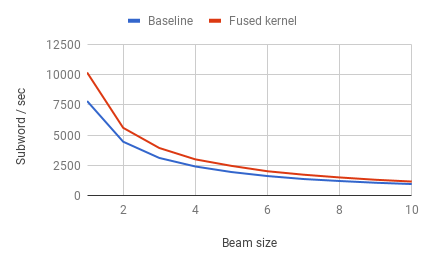
\includegraphics[scale=0.5]{beam-europarl.png}} 
\end{tabular}
\caption{Speed using the fused kernel (Europarl)}
\label{fig:beam-europarl}
\end{figure} 

\begin{figure}
\centering
\begin{tabular}{cc}
{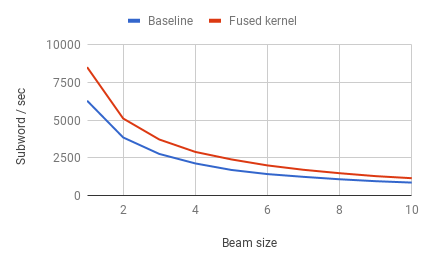
\includegraphics[scale=0.5]{beam-opensubtitles.png}} 
\end{tabular}
\caption{Speed using the fused kernel (OpenSubtitles)}
\label{fig:beam-opensubtitles}
\end{figure} 

\begin{figure}
\centering
\begin{tabular}{cc}
{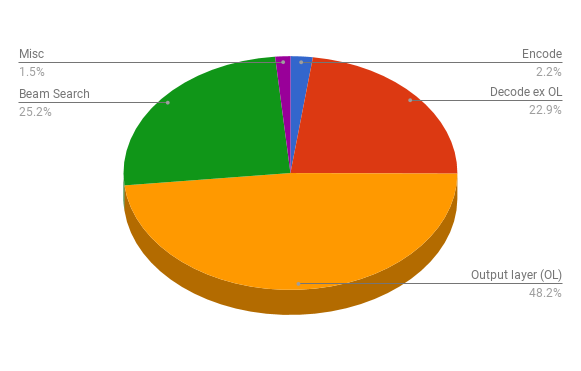
\includegraphics[scale=0.3]{pie-time-opensubtitles.png}} 
\end{tabular}
\caption{Proportion of time spent during translation (OpenSubtitles)}
\label{fig:pie-time-opensubtitles}
\end{figure} 


\subsection{Top-up Batching}

After some experimentation, we decided to top-up the decoding batch only when it is at least half empty, rather than whenever a sentence has completed.

The top-up batching and maxi-batching have similar goals of maximizing efficiency when translating batches of different lengths. Therefore, using both methods together gives limited gains, in fact, using top-up batching with maxi-batch slows of between 2\% to 18\% when translating the Europarl test set due to the overhead of using the algorithm, Figure~\ref{fig:topup-europarl}. When maxi-batching is inappropriate, using top-up batching alone matches the performance of maxi-batching, even being slightly faster when a small beam is used.

\begin{figure}
\centering
\begin{tabular}{cc}
{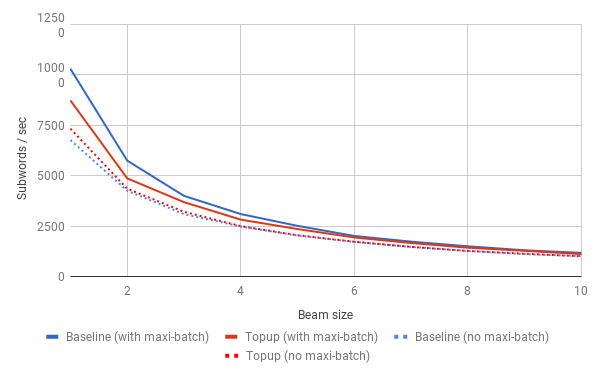
\includegraphics[scale=0.3]{topup-europarl.png}} 
\end{tabular}
\caption{Speed using top-up batching (Europarl)}
\label{fig:topup-europarl}
\end{figure} 

The results are better when translating the OpenSubtitles test set, Figure~\ref{fig:topup-opensubtitles}. The top-up batching does not harm performance when used with maxi-batching, even helping a little for small beams. However, top-up batching increases translation speed by up to 12\% when used alone.

\begin{figure}
\centering
\begin{tabular}{cc}
{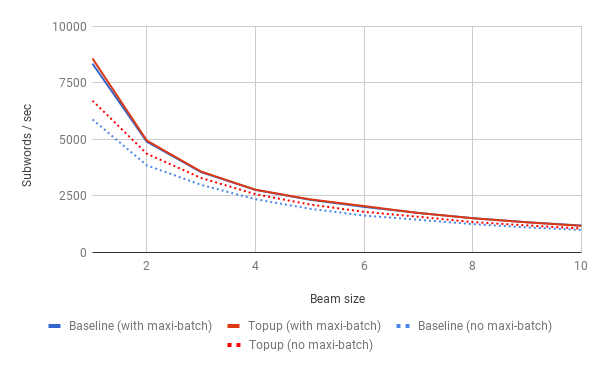
\includegraphics[scale=0.3]{topup-opensubtitles.png}} 
\end{tabular}
\caption{Speed using top-up batching (OpenSubtitles)}
\label{fig:topup-opensubtitles}
\end{figure} 

The gain from top-up batching is partially dependent on how much time the standard mini-batching algorithm spend decoding with a very small number of sentences as this is does not fully utilize the GPU cores. From Figure~\ref{fig:batch-size-small}, 20\% of the decoding iterations have less than 8 sentences remaining in the batch when translating the Europarl test test with maxi-batching. This figure is 50\% for the OpenSubtitles test set with no maxi-batching. The OpenSubtitles test set has a higher variance of sentence lengths relative to its average sentence length, which forces the mini-batch algorithm to continue decoding with a small number of sentences while the other sentences have already completed.

\begin{figure}
\centering
\begin{tabular}{cc}
{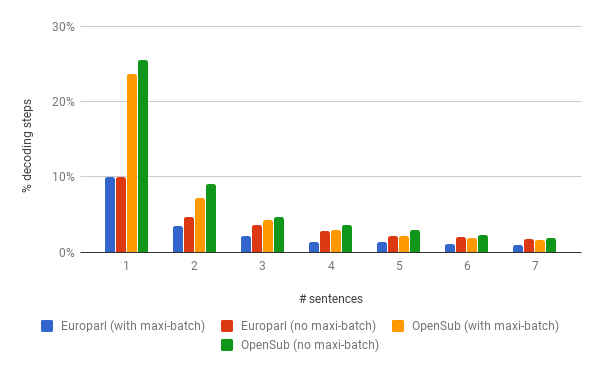
\includegraphics[scale=0.3]{batch-size-small.png}} 
\end{tabular}
\caption{Actual batch size during decoding}
\label{fig:batch-size-small}
\end{figure} 

\subsection{Cummulative Results}

Using both the fused kernel and top-up batching to translate led to a cummalative speed improvement of up to 57\% and 34\% for the OpenSubtitles and Europarl test set, respectively, when no maxi-batching is used, Figure~\ref{fig:cummulative-europarl} and Figure~\ref{fig:cummulative-opensubtitles}. With maxi-batching, the speed was up to 41\% and 21\%.

\begin{figure}
\centering
\begin{tabular}{cc}
{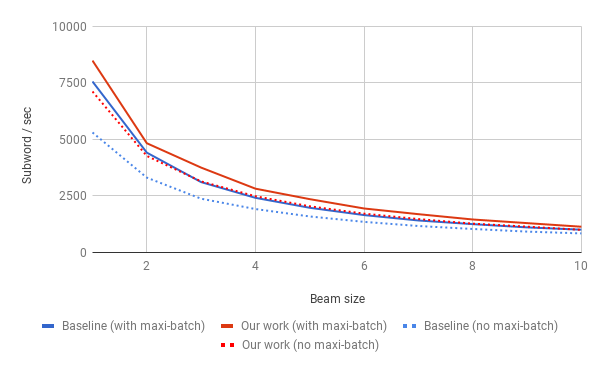
\includegraphics[scale=0.3]{cummulative-europarl.png}} 
\end{tabular}
\caption{Cummulative results (Europarl}
\label{fig:cummulative-europarl}
\end{figure} 

\begin{figure}
\centering
\begin{tabular}{cc}
{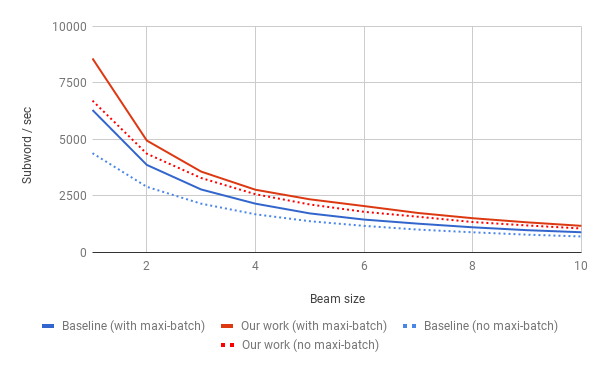
\includegraphics[scale=0.3]{cummulative-opensubtitles.png}} 
\end{tabular}
\caption{Cummulative results (OpenSubtitles}
\label{fig:cummulative-opensubtitles}
\end{figure} 

\section{Conclusion and Future Work}

We have presented two methods for faster deep-learning inference, targeted at neural machine translation. 

The first method focused on output layer of the neural network which accounts for a large part of the running time of the NMT model. By fusing the output layer with the beam search, we are able to increase translation speed by up to 41\%.

The second method replaces the mini-batching algorithm with one that avoids decoding with a small number of sentences, maximizing the parallel processing potential of GPUs. For certain scenarios, this increases translating  speed by up to 12\%.

For future work, we would like to apply our optimization for other NLP and deep-learning tasks. We are also interested in further optimization of the output layer in NMT, specifically the matrix multiplication which still takes up a significant proportion of the translation time.

%\section*{Acknowledgments}
%This work is sponsored by the Air Force Research Laboratory, prime contract FA8650-11-C-6160.  The views and conclusions contained in this document are those of the authors and should not be interpreted as representative of the official policies, either expressed or implied, of the Air Force Research Laboratory or the U.S. Government.

\bibliographystyle{apalike}
\bibliography{amta2016,mt,more}


\end{document}
\grid
\grid
